\documentclass[12pt]{article}

\usepackage[letterpaper,margin=0.75in]{geometry}
\usepackage[T1]{fontenc}
\usepackage{newtxtext}
\usepackage{lipsum}

% Figure stuff
\usepackage{floatrow}
\usepackage{multirow}
\usepackage{booktabs}
\setlength{\heavyrulewidth}{1.5pt}
\setlength{\abovetopsep}{4pt}

\usepackage{enumitem}
\setlist[enumerate]{itemsep=0mm}
%\usepackage{paralist}


% ToC
\usepackage{blindtext} 
\usepackage[linktocpage]{hyperref}
\usepackage{bookmark}
\usepackage[compact]{titlesec}

% bib
%\usepackage[round]{natbib}
\usepackage[square,sort,numbers]{natbib}

% Math Imports
\usepackage{amsmath, amssymb, bm, fancyhdr, sectsty, dsfont, mathtools}

% Tikz
\usepackage{tikz}
\usetikzlibrary{bayesnet}
\usetikzlibrary{arrows}
\usepackage{tikz}
\usepackage{tikz-dependency}
\usetikzlibrary{shapes.arrows, positioning, fit, bayesnet,
    arrows,backgrounds,patterns,matrix,calc,shadows,plotmarks,
    shapes,positioning,automata,positioning,spy,scopes,chains,decorations,decorations.pathreplacing}
\pgfdeclarelayer{background}
\pgfdeclarelayer{foreground}
\pgfsetlayers{background,main,foreground}

\usepackage{wrapfig}
\usepackage{comment}
\usepackage{subcaption}
\usepackage{cleveref}

\usepackage[font=small]{caption}

% Symbols
\newcommand\ind{\protect\mathpalette{\protect\independenT}{\perp}}
\def\independenT#1#2{\mathrel{\rlap{$#1#2$}\mkern2mu{#1#2}}}
\newcommand\norm[1]{\left\lVert#1\right\rVert}
\newcommand\set[1]{\left\{#1\right\}}

\newcommand\RNN{\mathrm{RNN}}
\newcommand\MLP{\mathrm{MLP}}
\newcommand\enc{\mathrm{enc}}
\newcommand\softmax{\mathrm{softmax}}

% Distributions
\newcommand{\Cat}{\mathrm{Cat}}
\newcommand\Expo{\mathrm{Expo}}
\newcommand\Bern{\mathrm{Bern}}
\newcommand\Pois{\mathrm{Pois}}
\newcommand\Bin{\mathrm{Bin}}
\newcommand\Unif{\mathrm{Unif}}
\newcommand\Betad{\mathrm{Beta}}
\newcommand\Gammad{\mathrm{Gamma}}
\newcommand\Geom{\mathrm{Geom}}
\newcommand\Logd{\mathrm{Logistic}}

\newcommand\E[1]{\mathbb{E}\left[#1\right]}
\newcommand\Es[2]{\mathbb{E}_{#1}\left[#2\right]}
\newcommand{\Var}{\mathrm{Var}}
\newcommand{\Cov}{\mathrm{Cov}}
\newcommand{\Cor}{\mathrm{Cor}}

% Bold stuff
\newcommand{\ba}{\mathbf{a}}
\newcommand{\bb}{\mathbf{b}}
\newcommand{\bc}{\mathbf{c}}
\newcommand{\bd}{\mathbf{d}}
\newcommand{\be}{\mathbf{e}}
\newcommand{\bg}{\mathbf{g}}
\newcommand{\bh}{\mathbf{h}}
\newcommand{\br}{\mathbf{r}}
\newcommand{\bs}{\mathbf{s}}
\newcommand{\bt}{\mathbf{t}}
\newcommand{\bv}{\mathbf{v}}
\newcommand{\bw}{\mathbf{w}}
\newcommand{\bx}{\mathbf{x}}
\newcommand{\by}{\mathbf{y}}
\newcommand{\bz}{\mathbf{z}}

% mathcal stuff
\newcommand{\mcD}{\mathcal{D}}

% math blackboard bold stuff
\newcommand{\R}{\mathbb{R}}
\newcommand{\C}{\mathbb{C}}
\newcommand{\Z}{\mathbb{Z}}
\newcommand{\N}{\mathbb{N}}
\newcommand{\Q}{\mathbb{Q}}


\DeclareMathOperator*{\argmin}{argmin}
\DeclareMathOperator*{\argmax}{argmax}

\titlespacing{\paragraph}{0pt}{*0}{*0}
%\setlength{\parskip}{-5mm plus1mm minus1mm}

\makeatletter
\newcommand{\subalign}[1]{%
  \vcenter{%
    \Let@ \restore@math@cr \default@tag
    \baselineskip\fontdimen10 \scriptfont\tw@
    \advance\baselineskip\fontdimen12 \scriptfont\tw@
    \lineskip\thr@@\fontdimen8 \scriptfont\thr@@
    \lineskiplimit\lineskip
    \ialign{\hfil$\m@th\scriptstyle##$&$\m@th\scriptstyle{}##$\crcr
      #1\crcr
    }%
  }
}
\makeatother

\usepackage{fancyhdr}
\pagestyle{fancy}

\usepackage[displaymath,mathlines]{lineno}
%\linenumbers

\title{Latent Information Extraction from Text}
\date{}
\begin{document}
\lhead{Justin Chiu}
\chead{2018 NDSEG Application}
\rhead{Research Proposal}
\maketitle{}

\vspace{-2cm}

{\small \textit{Keywords}:
information networks, natural language processing, information extraction, latent variable models }
\subsection*{Introduction}

%\paragraph{Relevance to Army BAA: II. A. c. iii. (3) Information Networks}
% Introduce knowledge graphs
In order to provide decision makers with the information
necessary to make informed choices as well as predict the effects of those choices,
we must have a structured representation of information to model the state of the world. \textit{Information networks} (as described in Army BAA: II. A. c. iii. (3)) provide a graphical representation of information and how it
propagates through a network.
I focus on knowledge graphs, information networks where each node contains a set of facts
about an entity and each edge describes how the facts in one node influence the facts in another.
% We allow self-loops
Knowledge graphs provide an intuitive and queryable representation of knowledge.
A decision maker may query the relevant nodes to gain situational awareness, and
when simulating a decision that alters the information in one node
the graph can easily propagate those changes by virtue of its representation.

%A knowledge graph aims to  represent a large number of facts and relationships,
%it is infeasible to specify these completely by hand.

Information extraction is the task of producing structured representations given unstructured text.
In the context of knowledge graphs,
information extraction is used to populate the nodes of
a knowledge graph conditioned on text.
%Figure~\ref{fig:d2t} is an example of a datum and text pair which may be used to
%train an information extraction system, inspired by the Rotowire dataset \citep{wiseman2017d2t}.
A typical approach to an information extraction system is the following pipeline:
(i) segment the text into mentions and values, (ii) align the mentions to an entity, a node in a knowledge graph, (iii) identify the relationships between segments.
The relationships between these segments entail facts. Given the large cost of obtaining annotations to train an extraction system,
a model that can perform well with fewer annotations is appealing.
%For example, consider the case where Figure~\ref{fig:boxscore} is missing all values %except for 
%Michael Jordan's name.
My proposal focuses on scenarios where there is a surplus of text but a lack of annotations,
making it difficult to train an extraction system.

\subsection*{Proposal}
In order to circumvent the cost of obtaining annotations, I propose to explore the use of text, rather than the facts, as the main source of learning signal for information extraction. This can be accomplished through the use of \textit{latent variable models} (LVMs), which are defined
by a generative process or recipe for how a dataset is generated.
%The benefit of using an LVM is two-fold:
%i) An LVM can learn in the semi-supervised or unsupervised setting,
%where only a few labels or no labels are provided respectively.
%This implies a model can be trained with missing facts.
%ii) LVMs provide a principled approach for propagating uncertainty %throughout the model.
An LVM for information extraction specifies the probabilistic relationship between a knowledge graph and the text. Such a model permits probabilistic queries such as (i) how likely a sentence is given a set of facts, as well as (ii) what the distribution over facts is given a text. Training an LVM relies on queries of type (i), while using the LVM for information extraction requires queries of type (ii). \textbf{My proposal is to develop a latent variable model that describes the process of generating text, where there is an abundance of data, based on information from a knowledge graph.} 

I will apply this model in the
semi-supervised information extraction setting
with the following goals:
\begin{enumerate}
\item Demonstrate that a conditional model of text can provide signal for training an information extraction model.
\item Show that we can achieve competitive performance on knowledge graph extraction with fewer annotations. 
\item Incorporate more linguistic signals and latent structure into the LVM to improve modeling performance.
\end{enumerate}
The model will perform sequence-wise generation of text using facts from the nodes of a knowledge graph.
This approach is inspired by the work of \citet{liang2009semalign}, who learn to align facts to text without supervision.
Their work relies on the insight that a model of text
provides signal for learning the alignments:
if the likelihood of a segment of text improves when moving from one alignment choice to a another,
then the new alignment is more likely to be correct given a suitably strong likelihood model. In my proposed LVM, I will extend this approach to a deep learning based model that incorporates state-of-the-art extraction and generation techniques.

%which aims to model not just the alignments from segments of text to nodes in a knowledge graph
%but also the values in the nodes themselves.
%I build on the formulation in \citet{liang2009semalign} by parameterizing our LVM
%with neural networks, drastically increasing the generative model's capacity.

%where the model learns to generate the values, record alignments, and finally the text
%conditioned on the given entities and types.


%Specifically, I propose the use of hidden semi-Markov models (HSMMs),
%used in \citet{liang2009semalign} as a conditional generative model for the
%task of aligning segments of text to nodes in a knowledge graph without supervision.
%\citet{liang2009semalign} rely on the insight that a conditional generative model of text
%provides signal for learning the alignments:
%if the likelihood of a segment of text improves when moving from
%one alignment choice to a another,
%then the new alignment is more likely to be correct given a suitably strong likelihood model.


%We present one instance of an LVM, outline how it can be used to obtain
%an information extraction model without direct supervision,
%and argue that the same approach can be applied in even more %ambitious settings.
%Our proposed LVM is a conditional generative model that specifies
%the relationship between data, specifically the entities and types, and text.
%We denote this model \texttt{Values}.
%Let $\by$ be the text, $\ba$ be a latent variable that represents the
%alignments from words to records,
%$\bv$ all the values in a datum of records,
%and $\be,\bt$ the entities and types respectively.



\subsection*{Detailed Approach}


\paragraph{Problem Setup}
To model the problem of information extraction,  
consider a dataset consisting of data and text pairs
$\set{(\br^{(1)}, \by^{(1)}),(\br^{(2)},\by^{(2)})\ldots}$.
Each datum $\br = \set{r_1,\ldots,r_N}$ is a set of $N$ records or facts, where each record $r = (e, t, v)$
is a tuple containing an entity, type, and value.
We denote the aggregated collection of any elements as a bold variable.
The datum $\br$ is a simple knowledge graph or information network. 
Each text $\by = y_1,y_2,\ldots$ is a sequence of tokens each from a vocabulary $V$. As an example consider a dataset consisting of summaries of basketball games $\by$ aligned with the respective statistics $\br$ of those games in Figure~\ref{fig:d2t}. 
Here there are three records and the statement $\by = $ ``michael jordan had 22 points and 12 rebounds as well as four blocks''. For this example, the process of information extraction is to infer 
the values $\bv$ of the records given the entities $\be$, types $\bt$, and the text $\by$.

\paragraph{Method}

\begin{figure}[t]
\centering
\floatbox[{\capbeside\thisfloatsetup{capbesideposition={left,top},capbesidewidth=4cm}}]{figure}[\FBwidth]
{\caption{An example of information extraction. The  generative process constructs the text from the given facts. The inference process aims to infer missing facts in curly braces.}
\label{fig:d2t}}
{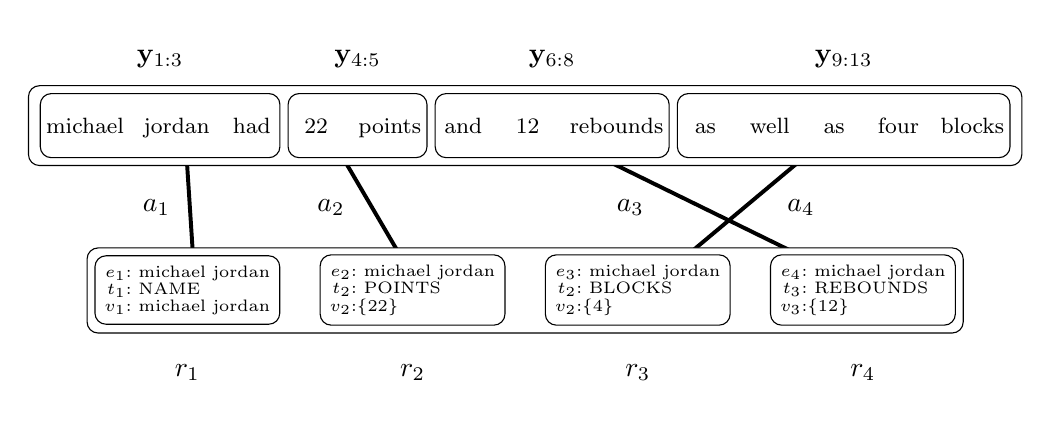
\begin{tikzpicture}[every node/.style={anchor=base,minimum size=8mm}]
\matrix (txt) [matrix of nodes, row sep=0.5em,column sep=0.05em,
    minimum width=0em, minimum height=1em, font=\footnotesize,ampersand replacement=\&,
    text height=.6em,text depth=.05em] {
      michael\& jordan \& % 1-2
      had \& % 3
      22\& points \& % 4-5
      and \& % 6
      12\& rebounds \& % 7-8
      as\& well\& as \& % 9-11
      four\& blocks % 12-13
    \\
   };
   \matrix (kb) [below=of txt,matrix of nodes, row sep=0.5em,column sep=1.5em,
    minimum width=0.5em, minimum height=1em, font=\small,ampersand replacement=\&] {
      $\subalign{e_1:& \textrm{ michael jordan}\\ t_1:& \textrm{ NAME}\\ v_1:& \textrm{ michael jordan}}$\&
      $\subalign{e_2:& \textrm{ michael jordan}\\ t_2:& \textrm{ POINTS}\\ v_2:& \set{22}}$\&
      $\subalign{e_3:& \textrm{ michael jordan}\\ t_2:& \textrm{ BLOCKS}\\ v_2:& \set{4}}$\&
      $\subalign{e_4:& \textrm{ michael jordan}\\ t_3:& \textrm{ REBOUNDS}\\ v_3:& \set{12}}$\\
    };
    \begin{scope}[on background layer]

    \draw[line width=0.5mm] ($(kb-1-1) + (0.1, 0)$) -- node[left] {$a_1$} ($(txt-1-2) + (0.1, 0)$);
    \draw[line width=0.5mm] ($(kb-1-2) + (0.1, 0)$) -- node[left,xshift=-1mm] {$a_2$} ($(txt-1-4) + (0.1, 0)$);
    \draw[line width=0.5mm] ($(kb-1-4) + (0.1, 0)$) -- node[left,xshift=-5mm] {$a_3$}  ($(txt-1-7) + (0.1, 0)$);
    \draw[line width=0.5mm] ($(kb-1-3) + (0.1, 0)$) -- node[right,xshift=3mm] {$a_4$} ($(txt-1-11) + (0.1, 0)$);

    \draw[rounded corners,fill=white] ($(kb-1-1.north west) +(-0.1,0.1)$) rectangle 
    node[yshift=-1cm]{} ($(kb-1-4.south east) +(0.1,-0.1)$);
    \draw[rounded corners,fill=white] ($(txt-1-1.north west) +(-0.1,0.1)$) rectangle  
    node[yshift=0.8cm]{} ($(txt-1-13.south east) +(0.1,-0.1)$);

    \draw[rounded corners,fill=white] (kb-1-1.north west) rectangle  node[ yshift =-1.1cm] {$r_1$} (kb-1-1.south east);
    \draw[rounded corners,fill=white] (kb-1-2.north west) rectangle  node[ yshift =-1.1cm] {$r_2$} (kb-1-2.south east);
    \draw[rounded corners,fill=white] (kb-1-3.north west) rectangle  node[ yshift =-1.1cm] {$r_3$} (kb-1-3.south east);
    \draw[rounded corners,fill=white] (kb-1-4.north west) rectangle  node[ yshift =-1.1cm] {$r_4$} (kb-1-4.south east);

    \draw[rounded corners, fill=white] (txt-1-1.north west)+(.05,0) rectangle 
    node[yshift=0.8cm]{$\by_{1:3}$}  ($(txt-1-3.south east) + (-.05, 0)$);
    \draw[rounded corners, fill=white] (txt-1-4.north west)+(.05,0) rectangle 
    node[yshift=0.8cm]{$\by_{4:5}$}  ($(txt-1-5.south east) + (-.05, 0)$);
    \draw[rounded corners, fill=white] (txt-1-6.north west)+(.05,0) rectangle 
    node[yshift=0.8cm]{$\by_{6:8}$}  ($(txt-1-8.south east) + (-.05, 0)$);
    \draw[rounded corners, fill=white] (txt-1-9.north west)+(.05,0) rectangle 
    node[yshift=0.8cm]{$\by_{9:13}$}  ($(txt-1-13.south east) + (-.05, 0)$);
    \end{scope}
\end{tikzpicture}}
\end{figure}
My proposed model is a conditional LVM that specifies the relationship between the different components of the data, specifically how the entities and types generate the text. Assume that the entities and relation types $\set{\be,\bt}$ of the knowledge graph are known.
Let $\ba = a_1,\ldots,a_T$ be a sequence of record indices,
such that each $a_t\in\set{1,\ldots,N}$. Each $a_t$ serves as an alignment from a specific record to a segment of text, as in Figure~\ref{fig:d2t}.
The model requires a generative process for
$\set{\by,\ba,\bv}$, i.e. the values, the text, and the alignments between the facts and text. This requires specifying: 
\[ p(\by, \ba, \bv \mid \be, \bt) = p(\bv \mid \be, \bt) \times p( \ba \mid \bv, \be, \bt) \times p(\by \mid \ba, \bv, \be, \bt).\]
The full generative process is the following:
\begin{enumerate}
\item Generate Prior Values: $p(\bv\mid\be,\bt)$.
For each entity and type pair in our datum of records, predict a prior value.
For example, given `michael jordan' and POINTS we predict 19.
Each value is predicted independently using a neural network over the entity $e$ and type $t$. 
\item Generate Record Alignments: $p(\ba \mid\bv,\be,\bt)$.
Conditioned on the knowledge graph, choose an ordered subset of records $\ba =a_1,\ldots,a_T$ for the text to describe. 
This sequence is predicted using a Markov chain parameterized with a neural network transition function that also takes into account a global encoding of the knowledge graph. 
\item Generate the Document: $p(\by\mid\ba,\bv,\be,\bt)$.
For each record selected as $a_i$, choose a sequence of words $\by_i = \set{y_{i1},\ldots,y_{iJ}}$ to describe the record
indicated by the alignment. This sequence is predicted using 
a recurrent neural network (RNN) that also takes into account 
an embedding of the current selected record. 
\end{enumerate}
This model is an instance of a hidden semi-Markov model (HSMM), a classical LVM that has been used for generation and extraction tasks. Our version extends the HSMM to incorporate methods from deep learning that have been shown to perform well on supervised extraction tasks.

To use this model for semi-supervised information extraction system we invert this generative process
to obtain the posterior distribution over alignments and values:
\begin{linenomath*}
$$
p(\ba,\bv\mid\by,\be,\bt)=\frac{p(\by,\ba,\bv\mid\be,\bt)}{p(\by\mid\be,\bt)}
=\frac{p(\by,\ba,\bv\mid\be,\bt)}{\sum_{\ba,\bv} p(\by,\ba,\bv\mid\be,\bt)}.
$$
\end{linenomath*}
Although the HSMM formulation allows the summation over alignments to be carried out efficiently,
the sum over value assignments is intractable.
I propose to instead apply variational inference,
where an approximation of the posterior distribution
is learned with a separate model.
% Can marginalize over alignments, so only a partial variational approximation is needed
The LVM and the approximate posterior are trained jointly 
by maximizing a lower bound on the log marginal likelihood of $\by$ with gradient-based methods.
The resulting approximate posterior  can be used independently of the 
original model as an information extraction system that gives a distribution over
values in a table of records and alignments from text to records.

\subsection*{Plan}

I plan to develop a system based on these ideas for information extraction with distant supervision. I will evaluate the approach on reduced annotation versions of standard information extraction benchmarks including the TAC KBP 2015 slot filling task and the TACRED dataset \citep{zhang2017slotfilling}.
The goal will be to demonstrate competitive performance on
extraction metrics such as precision, recall, and F1, while using as little supervision
as possible by ignoring subsets of the given data.
For example, we can allow the model to only learn from
subsets of the given values (or none at all).
Given success in that goal, the next step would be to extend the model
to capture more structure with the aim of boosting sample and label efficiency.
Possible extensions in this direction include coreference resolution \citep{haghighi2010coref},
learning the types of relations in a semi-supervised manner,
leveraging discourse structure to improve the model
\citep{sauper2009wiki}, explicitly modeling nuisance variables such as
author style \citep{hsu2017speech}, and incorporating multi-hop
reasoning in order to leverage relationships between entities
\citep{chen2018diva,rock17prove}.

Given admittance to the NDSEG Fellowship Program, I will evaluate the application of
LVMs to the problem of information extraction.
As a result of the digital age, the ubiquity of information networks as well as their 
enormous growth makes it clear that a method for training information extraction systems
with minimal supervision is a necessity.
I will push for scalable information extraction systems that require minimal supervision
by recasting information extraction as a text modeling problem.

\begin{comment}
\newpage
\section*{Outline}
\begin{enumerate}
\item Introduction
    \begin{enumerate}
    \item Relevance to BAA
        \begin{enumerate}
        \item Intro to information networks and KG
            \begin{enumerate}
            \item Information networks and decision making
            \item Specify knowledge graphs as the information networks we are interested in
            \item Brief outline of knowledge graphs, ie nodes are entities, contain sets of facts,
                edges specify relationships between facts (can include self-loops)
            \end{enumerate}
        \item Argument that KGs cannot be populated by hand. (Brief outline of methods for populating,
            no in-depth descriptions provided in this proposal)
            \begin{enumerate}
            \item Link prediction
            \item Multi-hop link prediction
            \item Corpora-based
            \end{enumerate}
        \item Proposal: train information extraction systems by recasting as a
            generative modeling problem.
        \end{enumerate}
    \item Background
        \begin{enumerate}
        \item We focus on information extraction, which is the task of producing structured
            representations of text.
        \item Define information extraction
            \begin{enumerate}
            \item The goal is to produce or fill in structured representations of information from
                a given unstructured text.
            \item A typical pipeline for information extraction includes
                text segmentation, named entity recognition, coreference resolution,
                relation extraction, and finally producing structured representations of the unlabeled text.
            \end{enumerate}
    \item Generative model
        \item If we have more text than labels, or at best noisy incomplete labels from heuristic methods...
        \item In this case, it is easier to do the inverse problem: learn to generate
            text from facts.
        \item We learn to generate text, which is the inverse of information extraction, with a generative model.
            We then use an algorithm called belief propagation to invert the
            generative process of the model to obtain an information extraction system.
        \item Benefits
            \begin{enumerate}
            \item stuff
            \end{enumerate}
        \end{enumerate}
    \item Recent advances in neural LVMs
        \begin{enumerate}
        \item Semi-supervised LVMs \citet{kingma2014ssvae}?
        \item Demonstrate that parameterization with a neural network does not affect computational
            complexity of inference.
        \item Then the same technique can be applied to model with more structure,
            as long as the graphical model itself permits tractable inference.
        \item In this proposal, we focus on the hidden semi-Markov model (HSMM),
            used in \citet{liang2009semalign} for the task of aligning segments of text to
            records in a knowledge base without supervision. 
        \item As in \citet{liang2009semalign}, we are interested in learning a generative model of text so that
            we can minimize the amount of supervision necessary for training an
            information extraction system.
        \item Also that although worse sample complexity, using an approximate posterior
            with monte carlo sampling achieves comparable performance.
        \end{enumerate}
    \end{enumerate}
\item Background and Notation
    \begin{enumerate}
    \item Formal notation for elements of the dataset
    \item Define the distribution we would like to learn: $p(z\mid y, x)$.
        $z$ and $x$ are placeholders and will change, but $y$ is always the text.
    \item Link to rotowire example
        (argument is that ACE is made up of ontonotes-like sentences, so all short-form)
    \item Clarify that the scope of posterior inference is very general.
    \end{enumerate}
\item Proposal
    \begin{enumerate}
    \item Outline approach
        \begin{enumerate}
        \item Choose a subset of available data as conditioning,
            and thus it is not modelled.
        \item The joint distribution of the remaining variables,
            both observed and unobserved, will be modelled.
        \end{enumerate}
    \item Link back to motivation. We want to scale information extraction
        by requiring less supervision.
    \item We present one model as an example, which we will serve as
        a starting point for the proposed research.
    \item Define generative model: HSMM as in \citep{liang2009semalign},
        and \citep{wiseman2018template}.
        The generative story (a picture would be helpful):
        \begin{enumerate}
        \item Fill in values
        \item Choose alignments
        \item Choose words
        \end{enumerate}
    \item Define IE as the distribution we would like to learn
        \begin{enumerate}
        %\item Align: $p(c\mid\by,\br)$
        \item Values: $p(c,\bv\mid\by,\be,\bt)$ (Just this one)
        %\item ??: $p()$
        \end{enumerate}
    \item We either use the posterior distribution of the conditional model
        or learn an approximation of it.
    \item Training and Inference
        \begin{enumerate}
        \item As we are dealing with large state spaces,
            we train with an approximate posterior in order to satisfy memory constraints.
        \item Highlight that the approx posterior is a SEPARATE model
            that can be used completely independently from generative model,
            i.e. we throw away generative model after training.
        \item We maximize a lower bound on the log marginal likelihood,
            called the evidence lower bound.
        \end{enumerate}
    \item Experiments, evaluation, and expectation
        \begin{enumerate}
        \item Evaluate on Rotowire.
        \item We evaluate \texttt{Values} using the precision, recall, and F1 score on the task
            of predicting the values associated with entities, otherwise known as slot-filling.
        \item What would success look like?
            \begin{enumerate}
            \item Competitive to supervised methods when supervision is available
            \item But able to be applied when supervision is not available
            \item Able to leverage lots of unlabeled data during training,
                and success would see a marked improvement over purely supervised methods
                as well as the purely supervised version of this model.
            \item Would provide explanations for the answers (ie segmentations).
            \end{enumerate}
        \item Also on ACE?
        \end{enumerate}
    \item Future work
        \begin{enumerate}
        \item Incorporate more structure into the generative model,
            for example entity tracking or coreference resolution \citet{haghighi2010coref}.
        \item Model more structure in the data, for example the edges between nodes
            in the knowledge graph \citet{chen2018diva}.
        \item `Multi-hop' reasoning, where we try to compose relationships to infer new ones,
            i.e. through unification \citet{chen2018diva,rock17prove}.
        \end{enumerate}
    \item Conclusion
        \begin{enumerate}
        \item Please accept!
        \item Recap: Minimal supervision IE systems so that they can scale to
            extracting information for large information networks from large bodies of text.
        \end{enumerate}
    \end{enumerate}
\end{enumerate}
\end{comment}

\newpage
\bibliographystyle{plainnat}
\bibliography{w}

\end{document}

